%\documentclass[handout,space,nooutcomes]{ximera}
\documentclass{ximera}

\graphicspath{
	{./}
	{ximeraTutorial/}
	{eulerCharacteristic/}
	{payingOffDebt/}
	{drugDecay/}
	}

\newenvironment{sectionOutcomes}{}{}


%\usepackage{wasysym}
%\newcommand{\pt}{\text{\smiley{}}}
\newcommand{\pt}{\bigstar}
\usepackage{tkz-euclide}
\usetikzlibrary{backgrounds} %% for boxes around graphs
\usetikzlibrary{shapes,positioning}  %% Clouds and stars
%\usetkzobj{all}
\usepackage{multicol}

%\usepackage[strict]{changepage}

\title{Complex Numbers}
\author{Brad Findell \and Bart Snapp}
\begin{document}
\begin{abstract}
Here we investigate complex numbers algebraically and geometrically.
\end{abstract}
\maketitle

\begin{question}
Which is better?  Explain. 
\begin{multipleChoice}
\choice{$\sqrt{9} = \pm 3$.} 
\choice[correct]{$\sqrt{9} = 3$.}
\choice{Either one is fine.}
\end{multipleChoice}
\begin{question}
Although it is true that both $3$ and $-3$ are ``square roots'' of $9$, the convention is that $\sqrt{9}=3$, so that the notation is unambiguous.  

When $a>0$, the notation $\sqrt{a}$ means the \emph{principal} square root of $a$, which is to say the positive one.  If $a<0$ or if $a$ is a non-real complex number, then the notation is less clear.

What do ``convention'' and ``unambiguous'' mean in the first paragraph? 
\end{question}

\end{question}


\begin{question}
\begin{enumerate}
\item Simplify $(3 + 4i) + (2 - 5i)$. $\answer{7-i}$
\item Multiply $(2 + 3i)$ and $(4 - i)$.  $\answer{11+10i}$
\item Find the modulus and argument of $-3 + 4i$.  Modulus: $\answer{5}$.  Argument: $\pi-\arctan(\frac{4}{3})$
\item Divide $\frac{5 + 2i}{1 - i}$ and write the result in standard form $a + bi$.   $\answer{\frac{3}{2}+\frac{7}{2}i}$
\end{enumerate}

%5. Solve $z^2 + 4z + 13 = 0$ and express the roots in terms of complex numbers.  

\end{question}

%### **Conceptual Questions**  
%1. Why are complex numbers necessary, and how do they extend the real number system?  
%2. Explain the geometric interpretation of multiplying two complex numbers.  
%3. What is the significance of the conjugate of a complex number in division?  
%4. How is Euler's formula $e^{i\theta} = \cos\theta + i\sin\theta$ connected to the polar representation of complex numbers?  
%5. Discuss the relationship between the modulus and argument of a complex number and its representation on the complex plane.


\begin{question}
Any complex number $z$ can be written $z=a+bi$, where $a$ and $b$ are real numbers and $i^{2}=-1$.  Its complex conjugate, $\overline{z}=a-bi$.   (Read ``z bar.'')

Do complex numbers include the real numbers?  
\begin{multipleChoice}
\choice[correct]{Yes.}
\choice{No.}
\choice{It depends.}
\end{multipleChoice}
Explain. 

\begin{question}
Correct! A complex number $a+bi$ is real when $b=\answer{0}$, so the complex numbers include the real numbers. A complex number is real exactly when $z=\overline{z}$. 

Some people use the phrase imaginary number to indicate a non-real complex number (i.e., $b\ne0$).  A complex number $a+bi$ is often called a pure imaginary number if $a=0$ and $b\ne\answer{0}$.  

\end{question}
\end{question}

\begin{question}

If we identify the complex number $a+bi$ with the ordered pair $(a,b)$, we can plot complex numbers as points (or vectors) on the complex plane.  The horizontal axis is call the real axis, abbreviated Re($z$); the vertical axis is called the imaginary axis, abbreviated Im($z$). 

\begin{image}
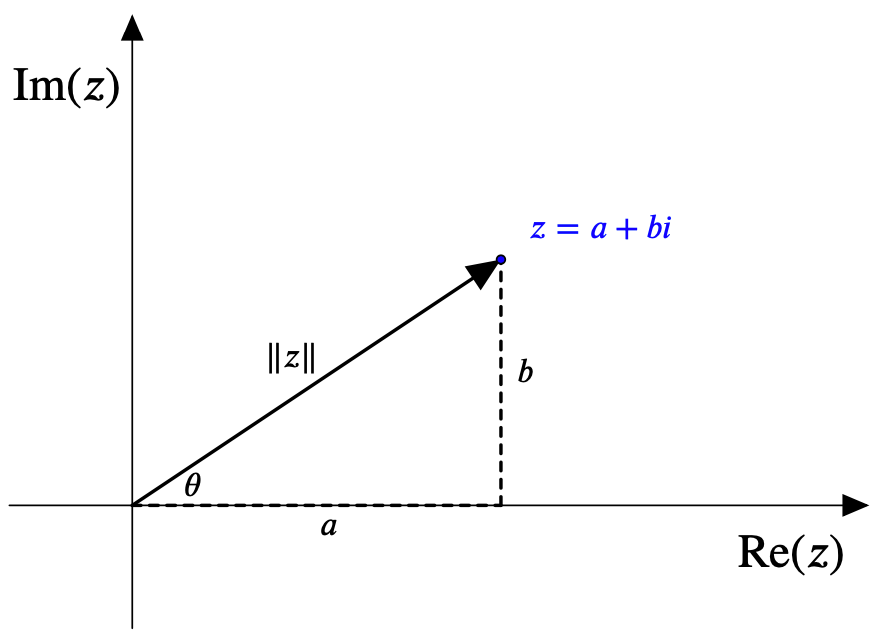
\includegraphics[scale=0.25]{complexNumber.png}
\end{image}

How do we find the magnitude of a complex number?  

\begin{question}
The magnitude of a complex number is its distance from origin:  $\|z\| =\sqrt{a^{2}+b^{2}}$.  It's also the length of the vector.  
\end{question}

\end{question}

\begin{question}

Suppose we let $r=\|z\| $, think of $z$ as a vector, and let $\theta$ denote the angle that vector makes with the positive real axis, then the complex number can be located with polar coordinates$\left(r;\theta\right)$.  (Some texts use a semicolon to distinguish polar coordinates from rectangular coordinates.)

\begin{image}
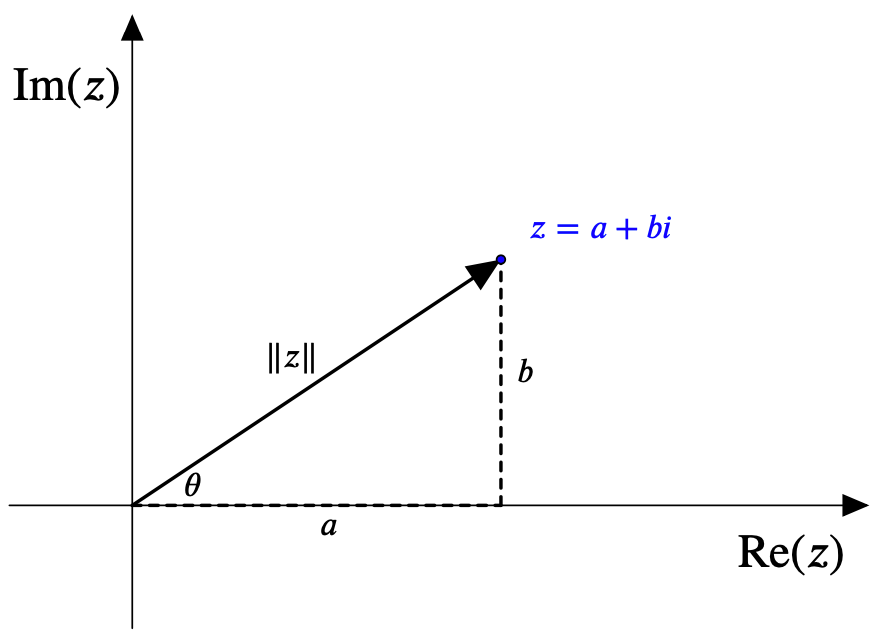
\includegraphics[scale=0.25]{complexNumber.png}
\end{image}

Write equations relating the rectangular coordinates $\left(a,b\right)$ and the polar coordinates.  
\begin{freeResponse}
\end{freeResponse}

\begin{question}
Yes, if a complex number has polar coordinates$\left(r;\theta\right)$and rectangular coordinates$\left(a,b\right),$ then $a=r\cos\theta$, $b=r\sin\theta$, $r^{2}=a^{2}+b^{2}$, and $\tan\theta=\frac{b}{a}$.  Practice converting between rectangular and polar coordinates.   
\end{question}
\end{question}

\begin{question}

Compute $z\overline{z}$.  What do you notice? 

Note: For $\overline{z}$, type \verb|\bar{z}| in text mode, select it, and press math mode.
\end{question}

\begin{question}
Yes, $z\overline{z}=\left(a+bi\right)\left(a-bi\right)=a^{2}+b^{2}=\|z\| ^{2}$.

What happens if $z$ is a real number? 
\begin{freeResponse}
\end{freeResponse}

\end{question}

\begin{question}
Yes, if $z$ is real, $b=0$, so $\|z\| =\sqrt{a^{2}+b^{2}}=\sqrt{a^{2}}=\left|a\right|$.  For this reason, some texts use absolute value symbols (rather than double bars) to indicate magnitudes of complex numbers.  

It is tempting to simplify as follows:$\sqrt{a^{2}}=a$.  What might you do to avoid this error? 
\begin{freeResponse}
\end{freeResponse}

\end{question}

\begin{question}
Think about adding $2+3i$ to every number in the complex plane.  How would that transform the plane?  Can you generalize to adding or subtracting any complex number? 

\begin{solution}
Adding $2+3i$ is a \wordChoice{\choice[correct]{translation}\choice{rotation}\choice{reflection}\choice{dilation}}
\end{solution}
 
\end{question}

\begin{question}
Think about multiplying every number in the complex plane by $3$.  How would that transform the plane?  

Hint: Try it for a few specific complex numbers.  Then generalize.  

\begin{solution}
Multiplying by $3$ is a \wordChoice{\choice{translation}\choice{rotation}\choice{reflection}\choice[correct]{dilation}} of the plane.  
\end{solution}

\end{question}

\begin{question}
Think about multiplying every number in the complex plane by $-1$.  How would that transform the plane?  

Hint: Try it for a few specific complex numbers.  Then generalize.  
\begin{solution}
Multiplying by $-1$ is a \wordChoice{\choice{translation}\choice[correct]{rotation}\choice{reflection}\choice{dilation}} of the plane.  
\end{solution}

\end{question}

\begin{question}
Think about multiplying every number in the complex plane by $i$.  How would that transform the plane?  

Hint: Try it for a few specific complex numbers.  Then generalize.  
\begin{freeResponse}
\end{freeResponse}

\end{question}


\begin{question}
Explore the geometry of complex multiplication. In the diagram, $v$ and $w$ are complex numbers, and $w=a+bi$, where $a$ and $b$ are real numbers. 

% See https://www.geogebra.org/m/f3dwskkd.

\begin{center}
\geogebra{f3dwskkd}{640}{480}
\end{center}

\begin{image}
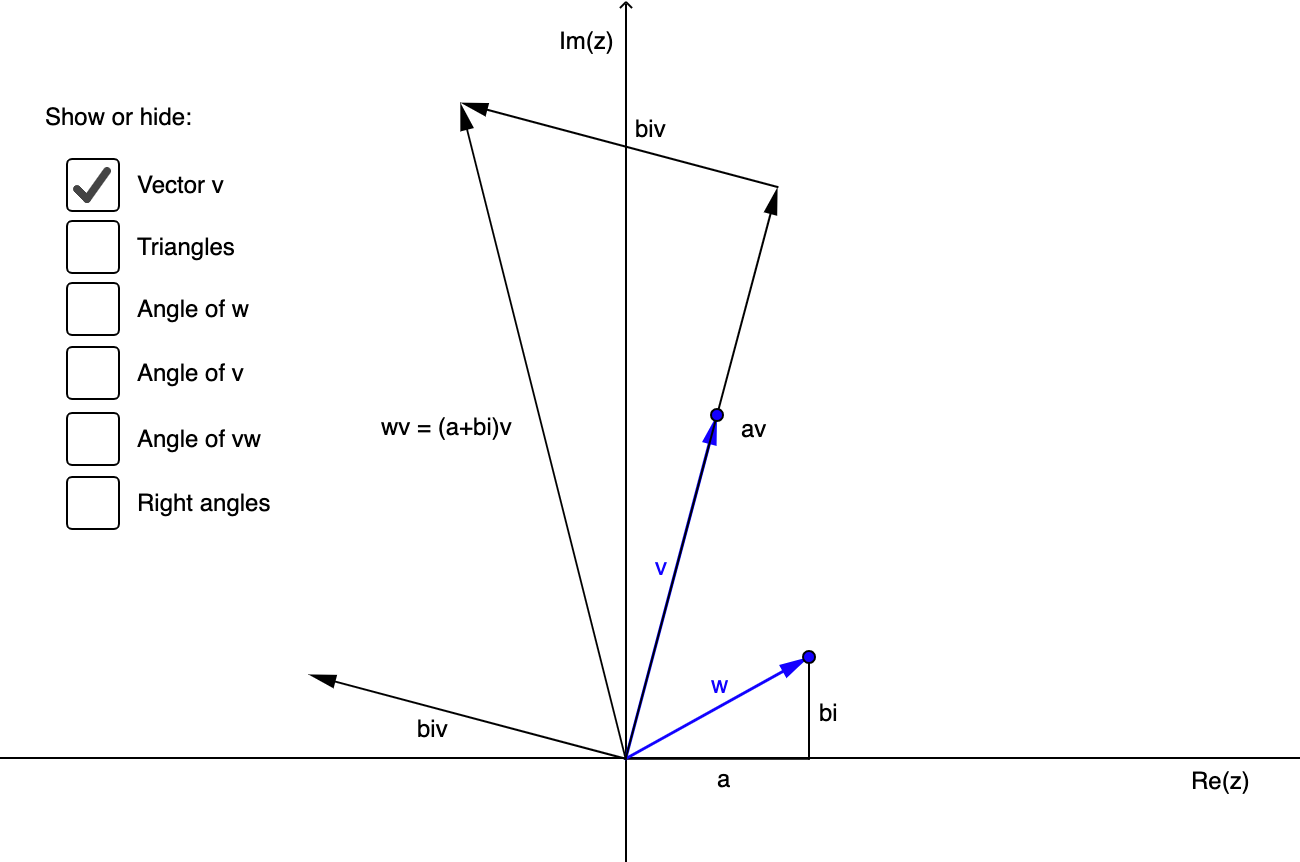
\includegraphics[scale=0.25]{complexMultiplication.png}
\end{image}

Build the product by considering the real and imaginary parts of $w$ separately.  In other words, because $w=\answer{a+bi}$, $wv=\answer{av+biv}$.  

\begin{question}
Why is $av$ as shown? Why is $biv$ as shown? Why is $wv$ as shown?


\begin{solution}
The vector $av$ scales $v$ by the real number $\answer{a}$, which appears to be greater than $1$ as shown. 

The vector $biv$ from the origin is a $\answer{90}$ degree rotation of $v$, scaled by the real number $\answer{b}$, with $0<b<1$ as shown.  

The second vector $biv$ is a translation of (and equal to) the first, positioned to illustrate \wordChoice{\choice{congruent}\choice[correct]{similar}\choice{scalene}} triangles.
\end{solution}

\begin{question}
Correct!  Why are they similar? What is the scale factor?
\begin{freeResponse}
The triangle with sides $av$, $biv$ and $wv$ is similar to the triangle with sides $a$, $bi$, and $w$.  They are similar by 
\wordChoice{\choice{SSS}\choice[correct]{SAS}\choice{ASA}} similarity, with the common right angles and scale factor $\| v\|$. 
\end{freeResponse}


How does the angle of the product $wv$ relate to the angles of $w$ and of $v$? Explain.
\begin{question}
The angle of $wv$ is the \wordChoice{\choice[correct]{sum}\choice{difference}\choice{product}} of the angles of $w$ and of $v$.  The angle of $wv$ is formed by adjacent angles from $v$ and from the similar triangle.  


How does the magnitude of the product $wv$ relate to the magnitudes of $w$ and $v$? Explain.
\begin{question}
The magnitude of the product is the \wordChoice{\choice{sum}\choice{difference}\choice[correct]{product}} of the magnitudes:  $\| wv\|=\| w\| \| v\|$.  
This follows because of the previously mentioned similar triangles with scale factor $\| v\|$.  

Summary of the results:  When multiplying complex numbers: \wordChoice{\choice{add}\choice{subtract}\choice[correct]{multiply}\choice{divide}} 
their magnitudes and \wordChoice{\choice[correct]{add}\choice{subtract}\choice{multiply}\choice{divide}} their angles.  
\end{question}

\end{question}
\end{question}
\end{question}

\end{question}

\begin{question}
You have seen Euler's formula.  

\[
e^{i\theta} = \sin\theta + i \cos\theta
\]

\end{question}


\end{document}
